\documentclass[sigconf,review]{acmart}
\usepackage{booktabs}
\usepackage{algorithm}
\usepackage{algorithmic}
\usepackage{subfigure}
\settopmatter{printacmref=false}

\setcopyright{rightsretained}

\acmConference[RecSys'18]{ACM Conference Series on Recommender Systems}{October 2nd}{Vancouver, Canada}
\acmYear{2018}
\copyrightyear{2018}

%\acmArticle{4}
%\acmPrice{15.00}
\begin{document}
\newcommand{\tabincell}[2]{\begin{tabular}{@{}#1@{}}#2\end{tabular}}
\title{Adaptive Model-based Feature Conjunction for CTR Prediction}
\begin{abstract}
Click-through rate (CTR) prediction is an important topic in recommender systems and computational advertising. As previous research indicates, a key point to maximize CTR is feature conjunction for making the training data more informative. Despite great progress, existing methods still fail to choose suitable settings of feature conjunction for the given data. In particular, a linear model on the pair-wise feature conjunction may overfit the training set if it is highly sparse. For such data a model based on low-rank latent matrices is shown to be more appropriate. Unfortunately, practitioners now face difficulties to decide when to use which. In this paper, we propose an adaptive framework to address the feature conjunction problem. Our proposed framework adaptively chooses effective models to do feature conjunction according to data properties. We offer a case for building feature conjunction based on feature-pair frequency. Efficient training as well as parameter selection are thoroughly investigated. We conduct comprehensive experiments to demonstrate the effectiveness of the adaptive model over existing models for CTR prediction on both benchmark and production data.\\\\
\textbf{KEYWORDS}\\
Recommender System, Machine learning, CTR, Feature Conjunction, Adaptive Model\\
\end{abstract}

\maketitle
\section{Introduction}

Recommendation has received much attention from both research and industry. The prediction of click-through rate (CTR) provides an important solution for recommending items to users. For example, some recommender systems require maximizing the number of clicks on the list of recommended items, a task that can be accomplished by ranking items according to CTR. On the other hand, online advertising systems aim to improve the revenue, which can be estimated as the CTR prediction multiplied by the received bid. Accurate CTR prediction is therefore essential for solving certain recommendation problems.

Some machine learning models have been applied in CTR prediction. Among them, logistic regression and its extensions have been widely used for this task \cite{Richardson:2007:PCE:1242572.1242643}. Suppose the data set consists of $m$ instances $\lbrace\boldsymbol{x}_i,y_i\rbrace_{i=1}^m$, where $\boldsymbol{x}_i$ is a data instance including $n$ user and item attributes, and $y_i\in\lbrace-1,1\rbrace$ is the associated label. That is, $y_i=1$ means the user clicks the item, and $y_i=-1$ otherwise. For any data point $\boldsymbol{x}$, if  $\boldsymbol{w}$ is the model vector and $\phi(\boldsymbol{w}, \boldsymbol{x})$ is the prediction function on whether $\boldsymbol{x}$ is clicked, logistic regression solves the following optimization problem:

\begin{equation}\label{1.1}
\min_{\boldsymbol{w}} \frac{\lambda}{2} \|\boldsymbol{w}\|_2^2+\sum_{i=1}^{m}\log(1+\exp(-y_i\phi(\boldsymbol{w},\boldsymbol{x}_i))),
\end{equation}
where $\lambda$ is the regularization parameter and the $\|\boldsymbol{w}\|_2^2$ term is used to avoid overfitting data. The second term in $(\ref{1.1})$ is an approximate sum of training errors by using the logistic loss.
In problem $(\ref{1.1})$, the $\phi$ function plays a very important role. Traditionally, a linear model (LM) is considered with $\phi(\boldsymbol{w}, \boldsymbol{x})=\boldsymbol{w}^{T}\boldsymbol{x}$. In a linear model, every feature corresponds to an individual weight, so relationship between features is not taken into account. However, as we observe in, for example, a commercial APP market, current app id combined with past downloaded apps is an important indicator in the prediction. Therefore, feature pair conjunction is crucial in CTR prediction and many works in real recommender systems are devoted to feature engineering, which aims to find effective feature interactions.

In data classification, second-order models are usually introduced to learn the feature conjunction instead of artificial feature interactions. As a widely adopted model, degree-2 polynomial (Poly2) \cite{Chang:2010:TTL:1756006.1859899} learns a particular weight for each possible feature conjunction. However, it has been known that Poly2 is not suitable for sparse data \cite{Juan:2016:FFM:2959100.2959134}, which are very common in real-world applications. Factorization machine (FM) \cite{5694074}\cite{Rendle:2012:FML:2168752.2168771} hence provides another way of feature conjunction under the sparse setting, which decomposes Poly2's one weight for each feature pair into the inner product of two short latent vectors associated with the feature pair. Furthermore, field-aware factorization machine (FFM) \cite{Juan:2016:FFM:2959100.2959134} has been proposed based on FM. FFM introduces the concept of fields, so feature fields are taken into consideration when combining a feature pair. All these models perform better than LM, indicating that feature conjunction is a key factor in predicting the CTR score.

It has been shown \cite{Juan:2016:FFM:2959100.2959134} that Poly2 and FM/FFM are useful for different types of data. In addition, one key observation we made is that the frequency of feature pairs in real data sets is not consistent, indicating that a single model cannot handle all real data sets. Therefore, having a model able to adapt to the data set seems to be essential for obtaining good performances.

In this paper, we propose a data adaptive framework to address the feature conjunction problem. We frame the problem as a model-based feature conjunction challenge. To find an appropriate feature conjunction for a feature pair, our framework adaptively chooses effective models based on data properties. As a case study, we then offer a novel adaptive model for building feature conjunctions in terms of the feature-pair frequency. Moreover, we search for the best hyperparameters to achieve the best adaptive setting. With the adaptive model, we significantly improve the performance of CTR prediction on multiple real-world data sets.

Our main contributions are summarized as follows:
\begin{itemize}
\item We propose a novel adaptive feature conjunction framework, consisting of the combination of several models. We specify the components of this framework, and justify how this framework works.
\item We offer a case study of the proposed framework by integrating Poly2 and FFM based on the feature-pair frequency. Moreover, we offer an effective optimization algorithm and provide a guideline on how to adjust the optimal hyperparameters in the model.
\item We evaluate our model on both public and our production data. Results show that our model gains improvement over existing models for CTR predcition.
\end{itemize}

\section{Existing Models: Poly2, FM and FFM}
\label{sec:FM}

Poly2 \cite{Chang:2010:TTL:1756006.1859899} effectively conducts feature conjunction by using the degree-2 polynomial expansion of features. This model learns a weight for each feature pair with the following $\phi$ function:
\begin{equation}
\label{poly2}
\phi_{\text{Poly2}}(\boldsymbol{w},\boldsymbol{x})=\sum_{j_1=1}^{n}\sum_{j_2=j_1+1}^{n} w_{h(j_1,j_2)}x_{j_1}x_{j_2},
\end{equation}
where $h(j_1,j_2)$ is a function encoding a feature pair, $x_{j_1}$ and $x_{j_2}$, into an index. Usually, all pairs are treated differently by, for example, \\
\begin{equation}
\label{hfunction}
h({j_1},{j_2})={j_1}n+{j_2}.
\end{equation}
However, if $x_{j_1}$ and $x_{j_2}$ rarely occur in the same instance, $w_{h({j_1},{j_2})}$ is learned by overfitting the few instances with $x_{j_1}x_{j_2}\neq0$. To avoid the overfitting situation, a hash function can be used to group some unrelated pairs together. Therefore, different pairs may share the same weight though selecting a suitable hash function may not be an easy task.

To address the issue of some rare $(x_{j_1}, x_{j_2})$ co-occurrences, in another model FM \cite{5694074}, the interaction between features is factorized into the product of latent factors. Each latent vector contains $k$ latent factors, where $k$ is a user-specified parameter. Then the $\phi$ function is as follows:
\begin{equation}
\label{fm}
\phi_{\text{FM}}(\boldsymbol{w},\boldsymbol{x}) = \sum_{j_1=1}^{n}\sum_{j_2=j_1+1}^{n} (\boldsymbol{w}_{j_1}\cdot\boldsymbol{w}_{j_2})x_{j_1}x_{j_2},
\end{equation}
where $\boldsymbol{w}_{j_1}$ (or $\boldsymbol{w}_{j_2}$) is a vector of $k$ latent factors. Because the updates of $\boldsymbol{w}_{j_1}$ and $\boldsymbol{w}_{j_2}$ are not restricted by the co-occurrence of feature pair $x_{j_1}$ and $x_{j_2}$ any more, the shortcoming of the Poly2 model may be alleviated.

Based on FM, FFM proposed in \cite{Juan:2016:FFM:2959100.2959134} introduces the concept of fields. FFM groups features to several fields.  For each feature, it has latent vectors to all fields. The $\phi$ function is as follows:
\begin{equation}
\label{ffm}
\phi_{\text{FFM}}(\boldsymbol{w},\boldsymbol{x}) = \sum_{j_1=1}^{n}\sum_{j_2=j_1+1}^n (\boldsymbol{w}_{j_1,f_2}\cdot\boldsymbol{w}_{j_2,f_1})x_{j_1}x_{j_2},
\end{equation}
where $f_1$ and $f_2$ are respectively the fields of $j_1$ and $j_2$. The idea is that in deciding the weight for $x_{j_1}x_{j_2}$, we use ${j_1's}$ associated latent vector on ${j_2's}$ field and ${j_2's}$ associated latent vector on ${j_1's}$ field.

To illustrate the way of feature conjunction in these models, we introduce an APP download example. Suppose an instance has three features and each feature is in a filed. The representation can be like 
\begin{center}
userdownload:map:1 gender:male:1 time:night:1,
\end{center}
where for example time is a field, night is a feature, and the feature value is one. Poly2 will encode a feature pair as $w_{h(\text{map,male})}$. For the same pair of features (\text{map}, \text{male}), FM has two latent vactors $\boldsymbol{w}_{\text{map}}$ and $\boldsymbol{w}_{\text{male}}$. It then uses $\boldsymbol{w}_{\text{map}}$$\cdot$$\boldsymbol{w}_{\text{male}}$ to get the weight of the feature conjunction. Moreover, FFM incorporates the concept of fields to the weight, making it as $\boldsymbol{w}_{\text{map,gender}}$$\cdot$$\boldsymbol{w}_{\text{male,userdownload}}$. Besides the same update way as FM, FFM groups the weight according to prior field information, providing a different way to do feature conjunction.

In all, both Poly2 and FM/FFM are used in CTR prediction. Poly2, as we have indicated, is useful for dense features (i.e., many training instances have non-zero values for the feature). In contrast, FM/FFM have been shown to be useful for sparse features. Hence, we could take both their advantages to do feature conjunction.

\section{Model-based feature conjunction}
We introduce our adaptive feature conjunction framework. Assume that a set of models, $\{\phi_1,\cdots,\phi_k\}$, is used for the same task. For each pair $(x_i,x_j)$, there are $k$ associated functions, denoted as 
\begin{equation}
\label{3.01}
f_1(i,j),\cdots, f_k(i,j)
\end{equation} 
Then we formulate our framework as:

\begin{equation}
\begin{split}
\label{3.1}
\phi(\boldsymbol{w},\boldsymbol{x}) =\sum_{i=1}^n \sum_{j=i+1}^n f_1(i,j)\phi_1(w,x_i,x_j)+\cdots  \\
+\sum_{i=1}^n \sum_{j=i+1}^n f_k(i,j)\phi_k(w,x_i,x_j).
\end{split}
\end{equation}
Usually only one of the $k$ values in (\ref{3.01}) is one and others are zeros, though more general settings can be considered. The intuition behind this new objective is that different feature pairs are routed to different models via their associated functions $f_1,\cdots,f_k$. Thus models suitable for different types of data can be effectively combined. While the concept of the proposed framework is simple, many issues must be addressed in order to make it practically viable. Next, we give some key points on this framework.

\subsection{What Models Could be Used?}
The models in (\ref{3.1}) should target to the same task, but provide different ways for feature conjunctions. For instance, both Poly2 and FFM model feature conjunctions in CTR prediction, so we can combine them together in our framework.

\subsection{How Could Models be Combined?}
Many potential priors could be encoded in $f(i,j)$, such as domain knowledge, feature pair frequency and so on. These functions can be in different forms. For example, a $0/1$ form indicates that under the given $(x_i,x_j)$, only some models are used. In contrast, if values are in the range [0,1], then a weighted combination is considered.

\section{An Adaptive Model for CTR prediction}

\label{sec:model}

We propose an adaptive model based on feature-pair frequency to illustrate our framework. From the given $m$ instances $\lbrace\boldsymbol{x}_i,y_i\rbrace_{i=1}^m$, we can introduce the %where $\boldsymbol{x}_i$ is a data instance including $n$ user and item attributes, and $y_i\in\lbrace-1,1\rbrace$ is the associated label. That is, $y_i=1$ means user click the item, $y_i=-1$ otherwise.
%We further introduce the 
feature density, which leads to $f$ functions for deciding the model to do feature conjunction. We make a number denoting how many times two features $x_{j_1}$ and $x_{j_2}$ both occur in the same training instance, which is the frequency of a feature pair. More formally
\begin{equation}
n_{j_1,j_2} := \lvert\lbrace\bigl((x_i)_{j_1},(x_i)_{j_2}\bigr) \mid (x_i)_{j_1}\ne0, (x_i)_{j_2}\ne0\rbrace\rvert.
\end{equation}

In our model, we suppose that different data sets have different feature-pair frequency distributions. For dense features, their $n_{j_1,j_2}$ is larger and we should consider the Poly2 models by following the discussion in Section \ref{sec:FM}. In contrast, for sparse features, $n_{j_1,j_2}$ is smaller and FM/FFM is more suitable.
As a result, we denote  a hyperparameter $val_{\text{thresh}}$ as a threshold value dividing the set of feature pairs. We define the following $0/1$ function:

\begin{equation}
\label{2.0}
\delta(x_{i_1},x_{j_2})=
\begin{cases}
1& \text{if}\, n_{j_1, j_2} < val_{\text{thresh}} \\
0& \text{otherwise}.
\end{cases}
\end{equation}

Based on the frequency, a feature pair is routed to one of the two models. We here consider Poly2 and FFM for dense and sparse feature pairs respectively, so the model is
\begin{equation}
\label{2.1}
\begin{split}
\phi_{\text{Adaptive}}&(\boldsymbol{w},\boldsymbol{x})= \\
&\sum_{j_1=1}^n\sum_{j_2=j_1+1}^n \biggl(\delta(x_{j_1},x_{j_2})\times(\boldsymbol{w}_{j_1,f_2}^\text{F}\cdot\boldsymbol{w}_{j_2,f_1}^\text{F})x_{j_1}x_{j_2} \\
&+(1-\delta(x_{j_1},x_{j_2}))\times w_{h(j_1,j_2)}^\text{P}x_{j_1}x_{j_2}\biggr), 
\end{split}
\end{equation}
where \\
%\begin{center}
\begin{align*}
\boldsymbol{w}=%\big[
\begin{bmatrix}
\begin{array}{c}
\boldsymbol{w}^\text{F}\\
\boldsymbol{w}^\text{P}
\end{array}
\end{bmatrix}.
%\big].
\end{align*}

%\end{center}
In (\ref{2.1}),\ $(\boldsymbol{w}_{j_1,f_2}^\text{F}\cdot\boldsymbol{w}_{j_2,f_1}^\text{F})x_{j_1}x_{j_2}$ is the FFM component and $w_{h(j_1,j_2)}^\text{P}x_{j_1}x_{j_2}$ is the Poly2 component. Note that in \eqref{2.1}, $\boldsymbol{w}^\text{F}_{j_1, f_2}, \boldsymbol{w}^\text{F}_{j_2, f_1} \in \mathbb{R}^k$, where $k$, as indicated in Section \ref{sec:FM}, is the latent dimension.

The $\phi_{\text{Adaptive}}$ function could be taken into the logistic regression model to get the final optimization problem
\begin{equation}\label{2.2}
\begin{split}
\min_{\boldsymbol{w}^{\text{F}},\boldsymbol{w}^{\text{P}}}\frac{\lambda_{\text{FFM}}}{2}\|\boldsymbol{w}^{\text{F}}\|_2^2 + \frac{\lambda_\text{Poly2}}{2}\|\boldsymbol{w}^\text{P}\|_2^2 &\\
+\sum_{i=1}^{m}\log(1+\exp(-y_i\phi_{\text{Adaptive}}(\boldsymbol{w},\boldsymbol{x}_i))),
\end{split}
\end{equation}
where $\lambda_{\text{FFM}}$ and $\lambda_{\text{Poly2}}$ are regularization paramters.

As in \cite{Beutel:2017:BGO:3038912.3052713}, we do hyperparameter optimization by as simple grid search, in which each run independently optimizes $\boldsymbol{w}$ under fixed hyperparameters. Specifically, we split a given data set $\mathcal{D}$ into three disjoint parts following the convention in evaluating prediction tasks. They are respectively the training set $\mathcal{D}^\text{Tr}$, the validation set $\mathcal{D}^\text{Val}$ and the test set $\mathcal{D}^\text{Te}$. The former two data sets are used to adjust the parameters in the model and we evaluate officially the final performance on the last one. Specifically, by changing $val_{\text{thresh}}$, $\lambda_\text{FFM}$ and $\lambda_\text{Poly2}$, the model achieving the best validation performance is used for the final training and evaluation.

\subsection{Optimization Method}

To solve the optimization problem (\ref{2.2}), we adopt a stochastic gradient method to enable an instance level gradient computation. We consider AdaGrad \cite{duchi2011adaptive} here, which is a variant of stochastic gradient methods commonly used in training a FFM model. At each step, a data point is sampled for updating the model vector $\boldsymbol{w}$. Because Poly2 and FFM are both considered, the sub-gradient vector contains two parts. If the feature interaction satisfies $\delta(x_{j_1},x_{j_2}) = 1$, then the corresponding sub-gradient components are:
\begin{align}
\label{2.5}
\boldsymbol{\mathit{g}}_{j_1,f_2}^\text{F} = \nabla_{\boldsymbol{w}_{j_1,f_2}^\text{F}}f(\boldsymbol{w}) = \lambda_\text{FFM}\cdot\boldsymbol{w}_{j_1,f_2}^\text{F} + \kappa\cdot\boldsymbol{w}_{j_2,f_1}^\text{F}x_{j_1}x_{j_2}, \\
\boldsymbol{\mathit{g}}_{j_2,f_1}^\text{F} = \nabla_{\boldsymbol{w}_{j_2,f_1}^\text{F}}f(\boldsymbol{w}) = \lambda_\text{FFM}\cdot\boldsymbol{w}_{j_2,f_1}^\text{F} + \kappa\cdot\boldsymbol{w}_{j_1,f_2}^\text{F}x_{j_1}x_{j_2}. \label{2.6}
\end{align}
Otherwise, the sub-gradient element is:
\begin{equation}
\label{2.9}
\mathit{g}_{j_1,j_2}^\text{P} = \nabla_{w_{h(j_1,j_2)}^\text{P}}f(w) = \lambda_\text{Poly2}\cdot w_{h(j_1,j_2)}^\text{P} + \kappa\cdot x_{j_1}x_{j_2}.
\end{equation}
In \eqref{2.5}-\eqref{2.9}, we have
\begin{equation}
\label{2.3.0}
\begin{aligned}
\kappa &= \frac{\partial\log(1+\exp(-y\phi_{\text{Adaptive}}(\boldsymbol{w},\boldsymbol{x})))}{\partial\phi_{\text{Adaptive}}(\boldsymbol{w},\boldsymbol{x})} \\
&= \frac{-y}{1+\exp(y\phi_{\text{Adaptive}}(\boldsymbol{w},\boldsymbol{x}))}.
\end{aligned}
\end{equation}

Then, the sums of squared gradient are also needed in AdaGrad. In the FFM part, the accumulated sum for each coordinate $d=1,\cdots,k$ is shown as follows.
\begin{align}
\label{2.3}
(G_{j_1,f_2}^\text{F})_d\gets(G_{j_1,f_2}^\text{F})_d+(\mathit{g}_{j_1,f_2}^\text{F})_d^2, \\
\label{2.4}
(G_{j_2,f_1}^\text{F})_d\gets(G_{j_2,f_1}^\text{F})_d+(\mathit{g}_{j_2,f_1}^\text{F})_d^2.
\end{align}
In the Poly2 part, the sum is accumulated as:
\begin{equation}
\label{2.11}
G_{h(j_1,j_2)}^\text{P}\gets G_{h(j_1,j_2)}^\text{P} + (\mathit{g}_{h(j_1,j_2)}^\text{P})^2.
\end{equation}

Finally, we update $\boldsymbol{w}_{j_1,f_2}^\text{F}$, $\boldsymbol{w}_{j_2,f_1}^\text{F}$ in FFM and $w_{h(j_1,j_2)}^\text{P}$ in Poly2 respectively via $\boldsymbol{G}_{j_1,f_2}^\text{F}$, $\boldsymbol{G}_{j_2,f_1}^\text{F}$ and $G_{h(j_1,j_2)}^\text{P}$.

\begin{align}
(w_{j_1,f_2}^\text{F})_d\gets(w_{j_1,f_2}^\text{F})_d-\frac{\eta}{\sqrt{(G_{j_1,f_2}^\text{F})_d}}(\mathit{g}_{j_1,f_2}^\text{F})_d \label{2.7}, \\
(w_{j_2,f_1}^\text{F})_d\gets(w_{j_2,f_1}^\text{F})_d-\frac{\eta}{\sqrt{(G_{j_2,f_1}^\text{F})_d}}(\mathit{g}_{j_2,f_1}^\text{F})_d \label{2.8},
\end{align}
and
\begin{equation}
\label{2.10}
w_{h(j_1,j_2)}^\text{P}\gets w_{h(j_1,j_2)}^\text{P} - \frac{\eta}{\sqrt{G_{h(j_1,j_2)}^\text{P}}}\mathit{g}_{h(j_1,j_2)}^\text{P},
\end{equation}
where $\eta$ is the learning rate. To begin the optimization process, we initialize $\boldsymbol{w^\text{F}}$ in the FFM component with values randomly sampled from a uniform distribution between $[0,1/\sqrt{k}]$, while $\boldsymbol{w^\text{P}}$ in the Poly2 component is initialized as $\boldsymbol{0}$. The initial values of $G$ are all set to one. The overall procedure is presented in Algorithm \ref{algo}.

\begin{algorithm}[ht]
\caption{Training Feature Frequency Adaptive Model}
\label{algo}
\begin{algorithmic}[1]
\renewcommand{\algorithmicrequire}{\textbf{Input}}
\REQUIRE{training set $\mathcal{D}^\text{Tr}$, test set $\mathcal{D}^\text{Te}$ and validation set $\mathcal{D}^\text{Val}$}
\STATE Initialize $G$, $\boldsymbol{w}^\text{F}$ and $w^\text{P}$.
\STATE Set $k$, $\lambda_\text{FFM}$, $\lambda_\text{Poly2}$, learning rate $\eta$ and epochs $T$.
\STATE Pre-compute the $n_{j_1,j_2}$ on $\mathcal{D}^\text{Tr}$
\STATE Give threshold value $val_\text{thresh}$.
\WHILE{$t<T$}
\FOR{$i \in \{1,\cdots,m\}$}
\STATE Sample a data point $(\boldsymbol{x},y)$
\STATE Calculate $\kappa$ by (\ref{2.3.0})
\FOR{$j_1\in$ non-zero terms in $\{1,\cdots,n\}$}
\FOR{$j_2\in$\ non-zero terms in $\{j_1,\cdots,n\}$}
\STATE Calculate $\delta$ according to (\ref{2.0})
\IF{$\delta(x_{j_1},x_{j_2}) = 1$}
\STATE Calculate the sub-gradient by (\ref{2.5}) and (\ref{2.6})
\FOR{$d\in \{1,\cdots,k\}$}
\STATE Update the gradient sum by (\ref{2.3}) and (\ref{2.4})
\STATE Update the model by (\ref{2.7}) and (\ref{2.8})
\ENDFOR
\ELSE
\STATE Calculate the sub-gradient by (\ref{2.9})
\STATE Update the gradient sum by (\ref{2.11})
\STATE Update the model by (\ref{2.10})
\ENDIF
\ENDFOR
\ENDFOR
\ENDFOR
\ENDWHILE
\end{algorithmic}
\end{algorithm}

\section{Experiments on CTR Data}
In this section, we demonstrate that the proposed adaptive model is effective for CTR prediction. First, we compare our model with other state-of-art models on several real-world data sets. Then, we conduct further analysis on the proposed method. In particular, because the key in our proposed model is the threshold value, we show how to locate an optimal threshold value with exploration on the data set.

\subsection{Experimental Settings}
We evaluate the effectiveness of our proposed adaptive model on three data sets. Two data sets are from Kaggle competitions, while another is a data set from our production system.
\begin{enumerate}
\item Criteo Dataset:\footnote{Criteo Data Set: http://www.kaggle.com/c/criteo-display-ad-chanllenge} This data set originates from a Kaggle competition. We use the processed set used in \cite{Juan:2016:FFM:2959100.2959134}.\footnote{Criteo Data Set: https://www.csie.ntu.edu.tw/$\sim$cjlin/libsvmtools/datasets/binary.html} We randomly split the data to 74\% for training, 13\% for validation, and 13\% for testing.
\item Avazu Dataset:\footnote{Avazu Data Set:http://www.kaggle.com/c/avazu-ctr-prediction} This set is from another Kaggle competition and we again use the processed form in \cite{Juan:2016:FFM:2959100.2959134}.\footnote{Avazu Data Set: https://www.csie.ntu.edu.tw/$\sim$cjlin/libsvmtools/datasets/binary.html} We split the data to 77\% for training, 10\% for validation, and 13\% for testing.
\item Company Dataset: This data set is from our service of providing personalized advertisement recommendation. We collect several days of users' click records, and let the last two days be used for validation and testing.
\end{enumerate}

The statistics of all data sets are summarized in Table \ref{tab1}.

\begin{table}[ht]
\caption{Statistics of data sets. Some information of the company data is not revealed. Density is the percentage of non-zeros in the data.}
\label{tab1}
\centering
\begin{tabular}{|c|c|c|c|c|}
  %\toprule
   \hline
  Data Set & \#instances & \#features & \#fields & density \\
  \hline
  criteo & 45,840,617 & 1,000,000 & 39 & 0.0039\%  \\
  \hline
  avazu & 40,428,967 & 1,000,000 & 15 & 0.0015\%  \\
  \hline
  company &tens of millions & $\le$500,000   &tens & $\leq$0.0050\% \\
  %\bottomrule
  \hline
\end{tabular}
\end{table}

Following most studies on CTR prediction, we consider the following logistic loss as our evaluation criterion.
\begin{equation}
\text{logloss}=\frac1{m}\sum_{i=1}^{m} \log(1+\exp(-y_{i}\phi(\boldsymbol{w}, \boldsymbol{x}_{i}))).
\end{equation}

We compare four models discussed in this work, where Poly2, FM and FFM serve as baselines to be compared with the proposed adaptive model.

\subsection{Results of the Comparison}
\label{sec:comparition}

We follow a rigorous setting to select parameters. The search range of each parameter is given as follows.
\begin{itemize}
\item $\eta$: the learning rate is used in the stochastic gradient  implementation for each model. We consider $\eta$ in $\{0.05,0.1,0.2\}$.
\item $\lambda$, $\lambda_{\text{FFM}}$, $\lambda_{\text{Poly2}}$: $\lambda$ is the regularization parameter for the three baseline models Poly2, FM and FFM, while for the adaptive model to combine Ploy2 and FFM, we have two parameters $\lambda_{\text{Poly2}}$ and $\lambda_{\text{FFM}}$. The search range is \{$0$, $10^{-6}$, $5\times10^{-6}$, $10^{-5}$, $5\times10^{-5}$, $10^{-4}$, $5\times10^{-4}$\}.
%\{0, $0.000001$, $0.000005$, $0.00001$, $0.00005$, $0.0001$, $0.0005\}$.
\item $t$: this parameter is the number of epochs for running the stochastic gradient method. We record the number of epochs when the logloss of the validation set stops decreasing. We then use the obtained $t$ as the stopping condition in training a model for prediction.
\item $val_{\text{thresh}}$: this parameter is used only in the proposed adaptive model for choosing between Poly2 and FFM. The range considered is between $0$ and
\begin{equation}
\label{5.0.1}
\max_{j_1,j_2} n_{j_1,j_2} +1.
\end{equation}
We then check $val_{\text{thresh}}$ by multiplying (\ref{5.0.1}) and ratios in a decreasing geometric sequence \{$1.0$,$0.0822$,$0.0067$,$0.0006$,$4.5\times10^{-5}$,$3.7\times10^{-6}$,$3.0\times10^{-7}$,$0.0$\}.

\item $k$: $k$ is the number of latent dimension for FM, FFM and our adaptive model. For Criteo and Avazu sets, we consider the same $k$ values used in \cite{Juan:2016:FFM:2959100.2959134}. For the company set, we consider $k$ values through grid search. 
\end{itemize}

\begin{table*}[!htb]
	\centering
	\caption{ Test logloss of using various models. The best logloss is underlined. We also present parameters of Criteo and Avazu selected from the validation procedure. The parameters of the Company set are omitted because of the company policy.}
	\label{tab2}
	\begin{tabular}{|c|c|c|c|c|c|}
		\hline
		Model&\multicolumn{2}{c|}{Criteo}&\multicolumn{2}{c|}{Avazu}&\multicolumn{1}{c|}{Company} \\
		\cline{2-6}
		&parameters&LogLoss&parameters&LogLoss&LogLoss\\
		\hline
		Poly2&$\eta$=0.1, $\lambda$=$10^{-6}$, $t$=15&0.44866&$\eta$=0.1, $\lambda$=$10^{-5}$, $t$=11&0.39783&0.004941 \\
		\hline
		FM&$\eta$=0.05, $\lambda$=$5\times10^{-5}$, $t$=9, $k$=100&0.44795&$\eta$=0.05, $\lambda$=$10^{-4}$, $t$=6, $k$=100&0.39852&0.005067 \\
		\hline
		FFM&$\eta$=0.1, $\lambda$=$10^{-5}$, $t$=10, $k$=4&0.44603&$\eta$=0.1, $\lambda$=$10^{-5}$, $t$=4, $k$=4&0.39622&0.004946 \\
		\hline
		Adaptive&\tabincell{c}{$\eta$=0.2, $t$=14, $k$=4, $val_{\text{thresh}}$ =22000,\\$\lambda_{\text{FFM}}$ =$5\times10^{-5}$, $\lambda_{\text{Poly2}}$ =0.0}&\underline{0.44565}&\tabincell{c}{$\eta$=0.2, $t$=4, $k$=4, $val_{\text{thresh}}$=8000, \\$\lambda_{\text{FFM}}$=$10^{-4}$, $\lambda_{\text{Poly2}}$=$10^{-6}$}&\underline{0.38779}&\underline{0.004934} \\
		\hline
	\end{tabular}
\end{table*}

Parameters achieving the best logloss are used for training the model to predict the test set. In Table \ref{tab2} we list parameters selected for each approach. The test logloss of different approaches is given in Table \ref{tab2}. Results show that under suitable thresholds to choose between Poly2 and FFM, the adaptive model performs the best on all data. This observation seems to indicate that different data sets have different degrees of sparsity, and a single model for feature conjunction could not always perform well.

\begin{table}[ht]
	\caption{In the adaptive framework, the percentage of pairs assigned to Poly2 and FFM models. Notice that we check all non-zero $(x_i)_{j_1}$ $(x_i)_{j_2}$, ${\forall}$ $i$, $j_1$, $j_2$.}
	\label{tab3}
	\centering
	\begin{tabular}{|c|c|c|}
		\hline
		Data Set & Poly2 & FFM  \\
		\hline
		Criteo & 60.83\% & 39.17\%  \\
		\hline
		Avazu &  22.32\% & 77.68\%  \\
		\hline
		Company & 67.54\% & 32.46\%  \\
		\hline
	\end{tabular}
\end{table}

To further illustrate the effectiveness of an adaptive model, in Table \ref{tab3}, by checking all non-zero valued pairs in the training set, we present the percentage of pairs assigned to Poly2 and FFM models. Results indicate that for the company set, the Poly2 model covers a higher percentage of pairs. Interestingly, this set is denser than the other two sets; see the density presented in Table \ref{tab1}. Further, when a single model is used, Poly2 is better than FFM. In contrast, for highly sparse sets Criteo and Avazu, FFM is superior to Poly2. Therefore, an adaptive model can rightly choose a more suitable model for each pair and leads to better performances regardless of the data sparsity.

\begin{table}
	\caption{Validation logloss under different $val_{\text{thresh}}$ values in the adaptive model. The Criteo set is used.}
	\label{tab4}
	\centering
	\begin{tabular}{|c|c|}
		\hline
		$val_{\text{thresh}}$&Logloss \\
		\hline
		0&0.44257 \\
		\hline
		12&0.44192 \\
		\hline
		148&0.44070 \\
		\hline
		1810&0.43900\\
		\hline
		22,000&0.43792 \\
		\hline
		268,000&0.43844\\
		\hline
		3,270,000&0.43848 \\
		\hline
		39,800,000&0.43861\\
		\hline
	\end{tabular}
\end{table}

\subsection{Further Analysis}

To confirm that the proposed adaptive model can choose the right model for each feature pair, we conduct some additional experiments. To begin, we check the threshold $val_{\text{thresh}}$, which is the most important parameter of the proposed adaptive model. By considering the Criteo data set, we check the test logloss by varying $val_{\text{thresh}}$. To connect to the validation process of finding the best $val_{\text{thresh}}$, for the experiment we use the Cirteo training set for training, while the validation set for prediction. Other parameters are fixed as values shown in Table \ref{tab2}. Note that when $val_{\text{thresh}} = 0$ and $max(n_{x_i,x_j})+1$, the adaptive model degenerates to Poly2 and FFM respectively under the setting of other parameters. Results in Table \ref{tab4} show that as $val_{\text{thresh}}$ increases, the logloss decreases. However, after a certain $val_{\text{thresh}}$ value, the test logloss starts increasing. This result indicates that the use of $val_{\text{thresh}}$ enables our model to adapt with the feature frequency.

We further check if the selected $val_{\text{thresh}}$ from a validation procedure leads to a clear separation of sparse and dense feature pairs. To this end, we check the distribution of the feature-pair frequencies $n_{j_1,j_2}$:
\begin{equation}
\begin{split}
prob_{m}=\frac{|\{(j_1,j_2)|n_{j_1,j_2} = m\}|}{\sum_{\overline{m}}|\{(j_1,j_2)|n_{j_1,j_2}= \overline{m}|\}},
\end{split}
\end{equation}
where
\begin{center}
%$\max\limits_{j_1,j_2} n_{j_1,j_2} +1$.
%$m$ = \{$1$,\cdots,$\max\limits_{j_1,j_2}$ $n_{j_1,j_2}$ +$1$\}.\\
$m = \{1,\cdots,\max\limits_{j_1,j_2} n_{j_1,j_2}\}$.\\
\end{center}
The relationship between $n_{j_1,j_2}$ and $prob_{m}$ is presented in Figure \ref{fig.1}.

\begin{figure}
	\centering
	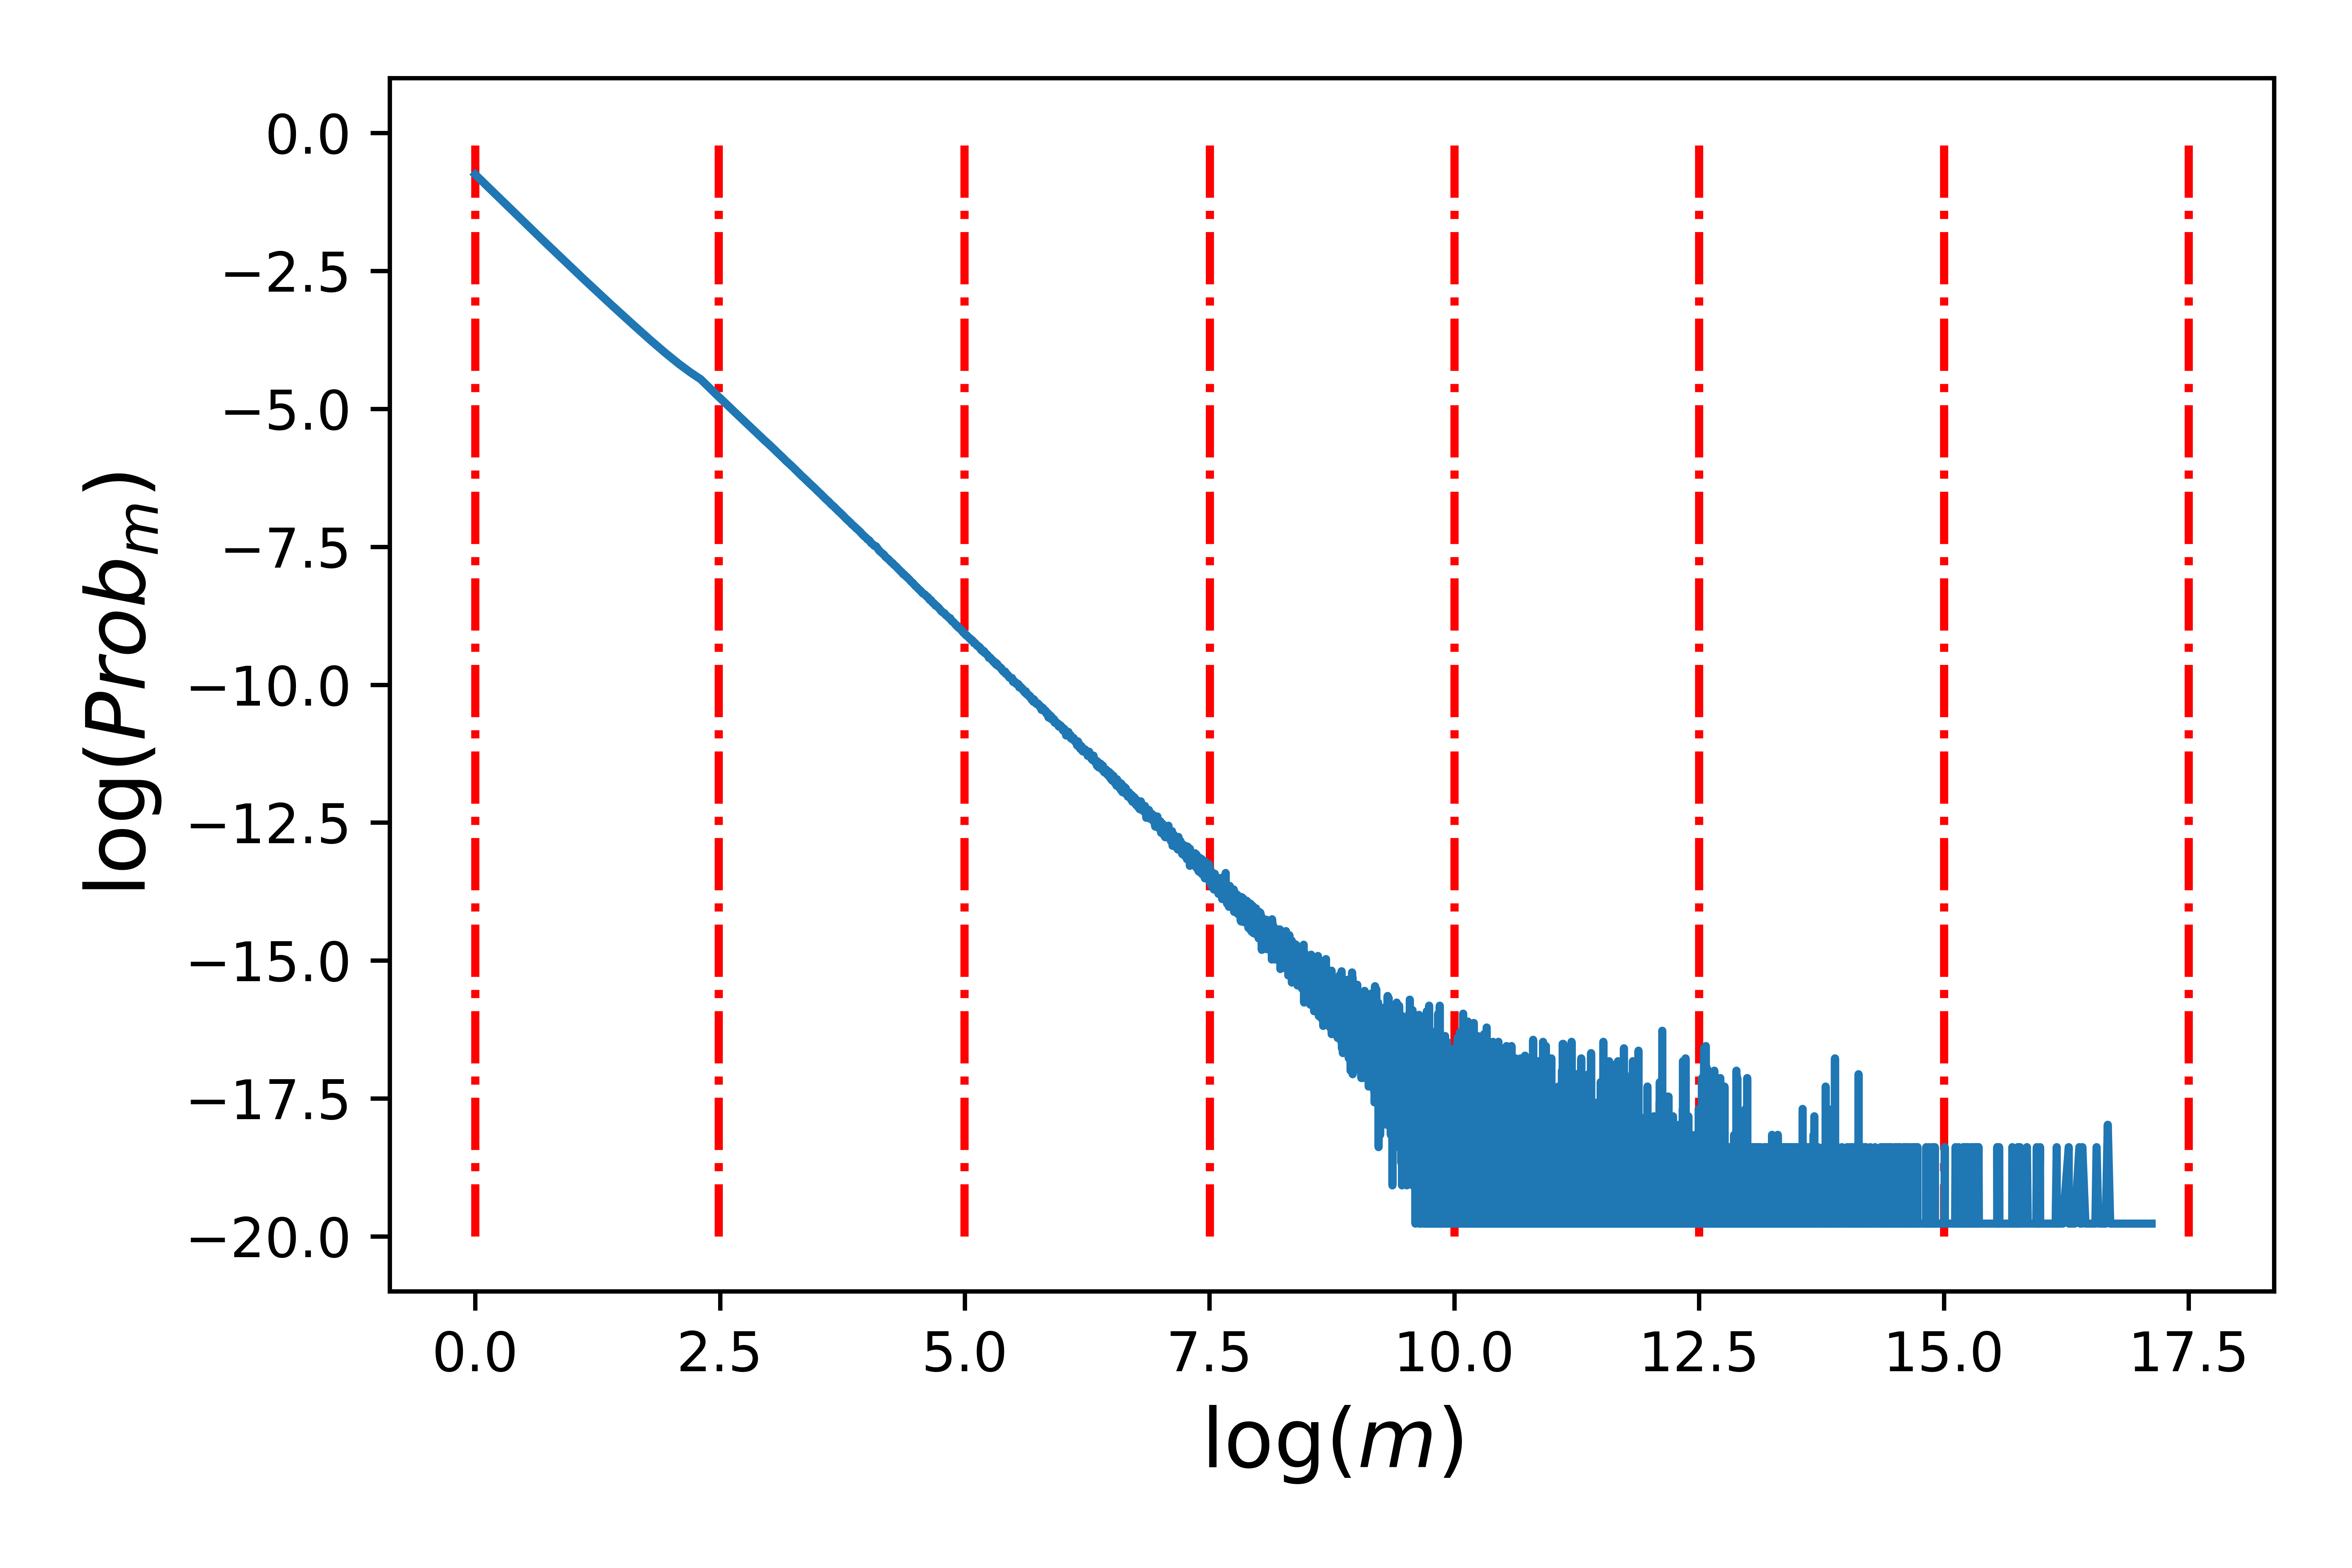
\includegraphics[width=0.5\textwidth]{criteo-thresh.png}
	\caption{Distribution of feature-pair frequency. Both axes are log-scaled. Vertical lines correspond to $val_{\text{thresh}}$ values used in Table.\ref{tab4}}
	\label{fig.1}
\end{figure}

From Figure \ref{fig.1}, $prob_{m}$ is larger when $m$ is small, indicating that many feature pairs occur a small number of times. This situation is reasonable because the set is very sparse. However, in the figure we observe that some pairs occur very frequently. For this set, dense and feature pairs can be well separated at around $\log(m)=10$. Interestingly, this cutting point corresponds to the smallest validation logloss in Table \ref{tab4}. Thus the validation procedure effectively finds a good $val_{\text{thresh}}$ to optimally combine Poly2 and FFM. To see if our method is equally effective for other data sets, in Figure \ref{fig.2}. we give the distribution of feature-pair frequencies for the other two sets, Avazu and Company. In the figure of each set, we draw a vertical line to indicate the $val_{\text{thresh}}$ that leads to the best validation logloss. Clearly, the obtained value rightly separates dense and sparse feature pairs. Then suitable models can be applied accordingly.

\begin{figure}
	\centering
	\subfigure[Avazu set]{
		\begin{minipage}[b]{0.5\textwidth}
			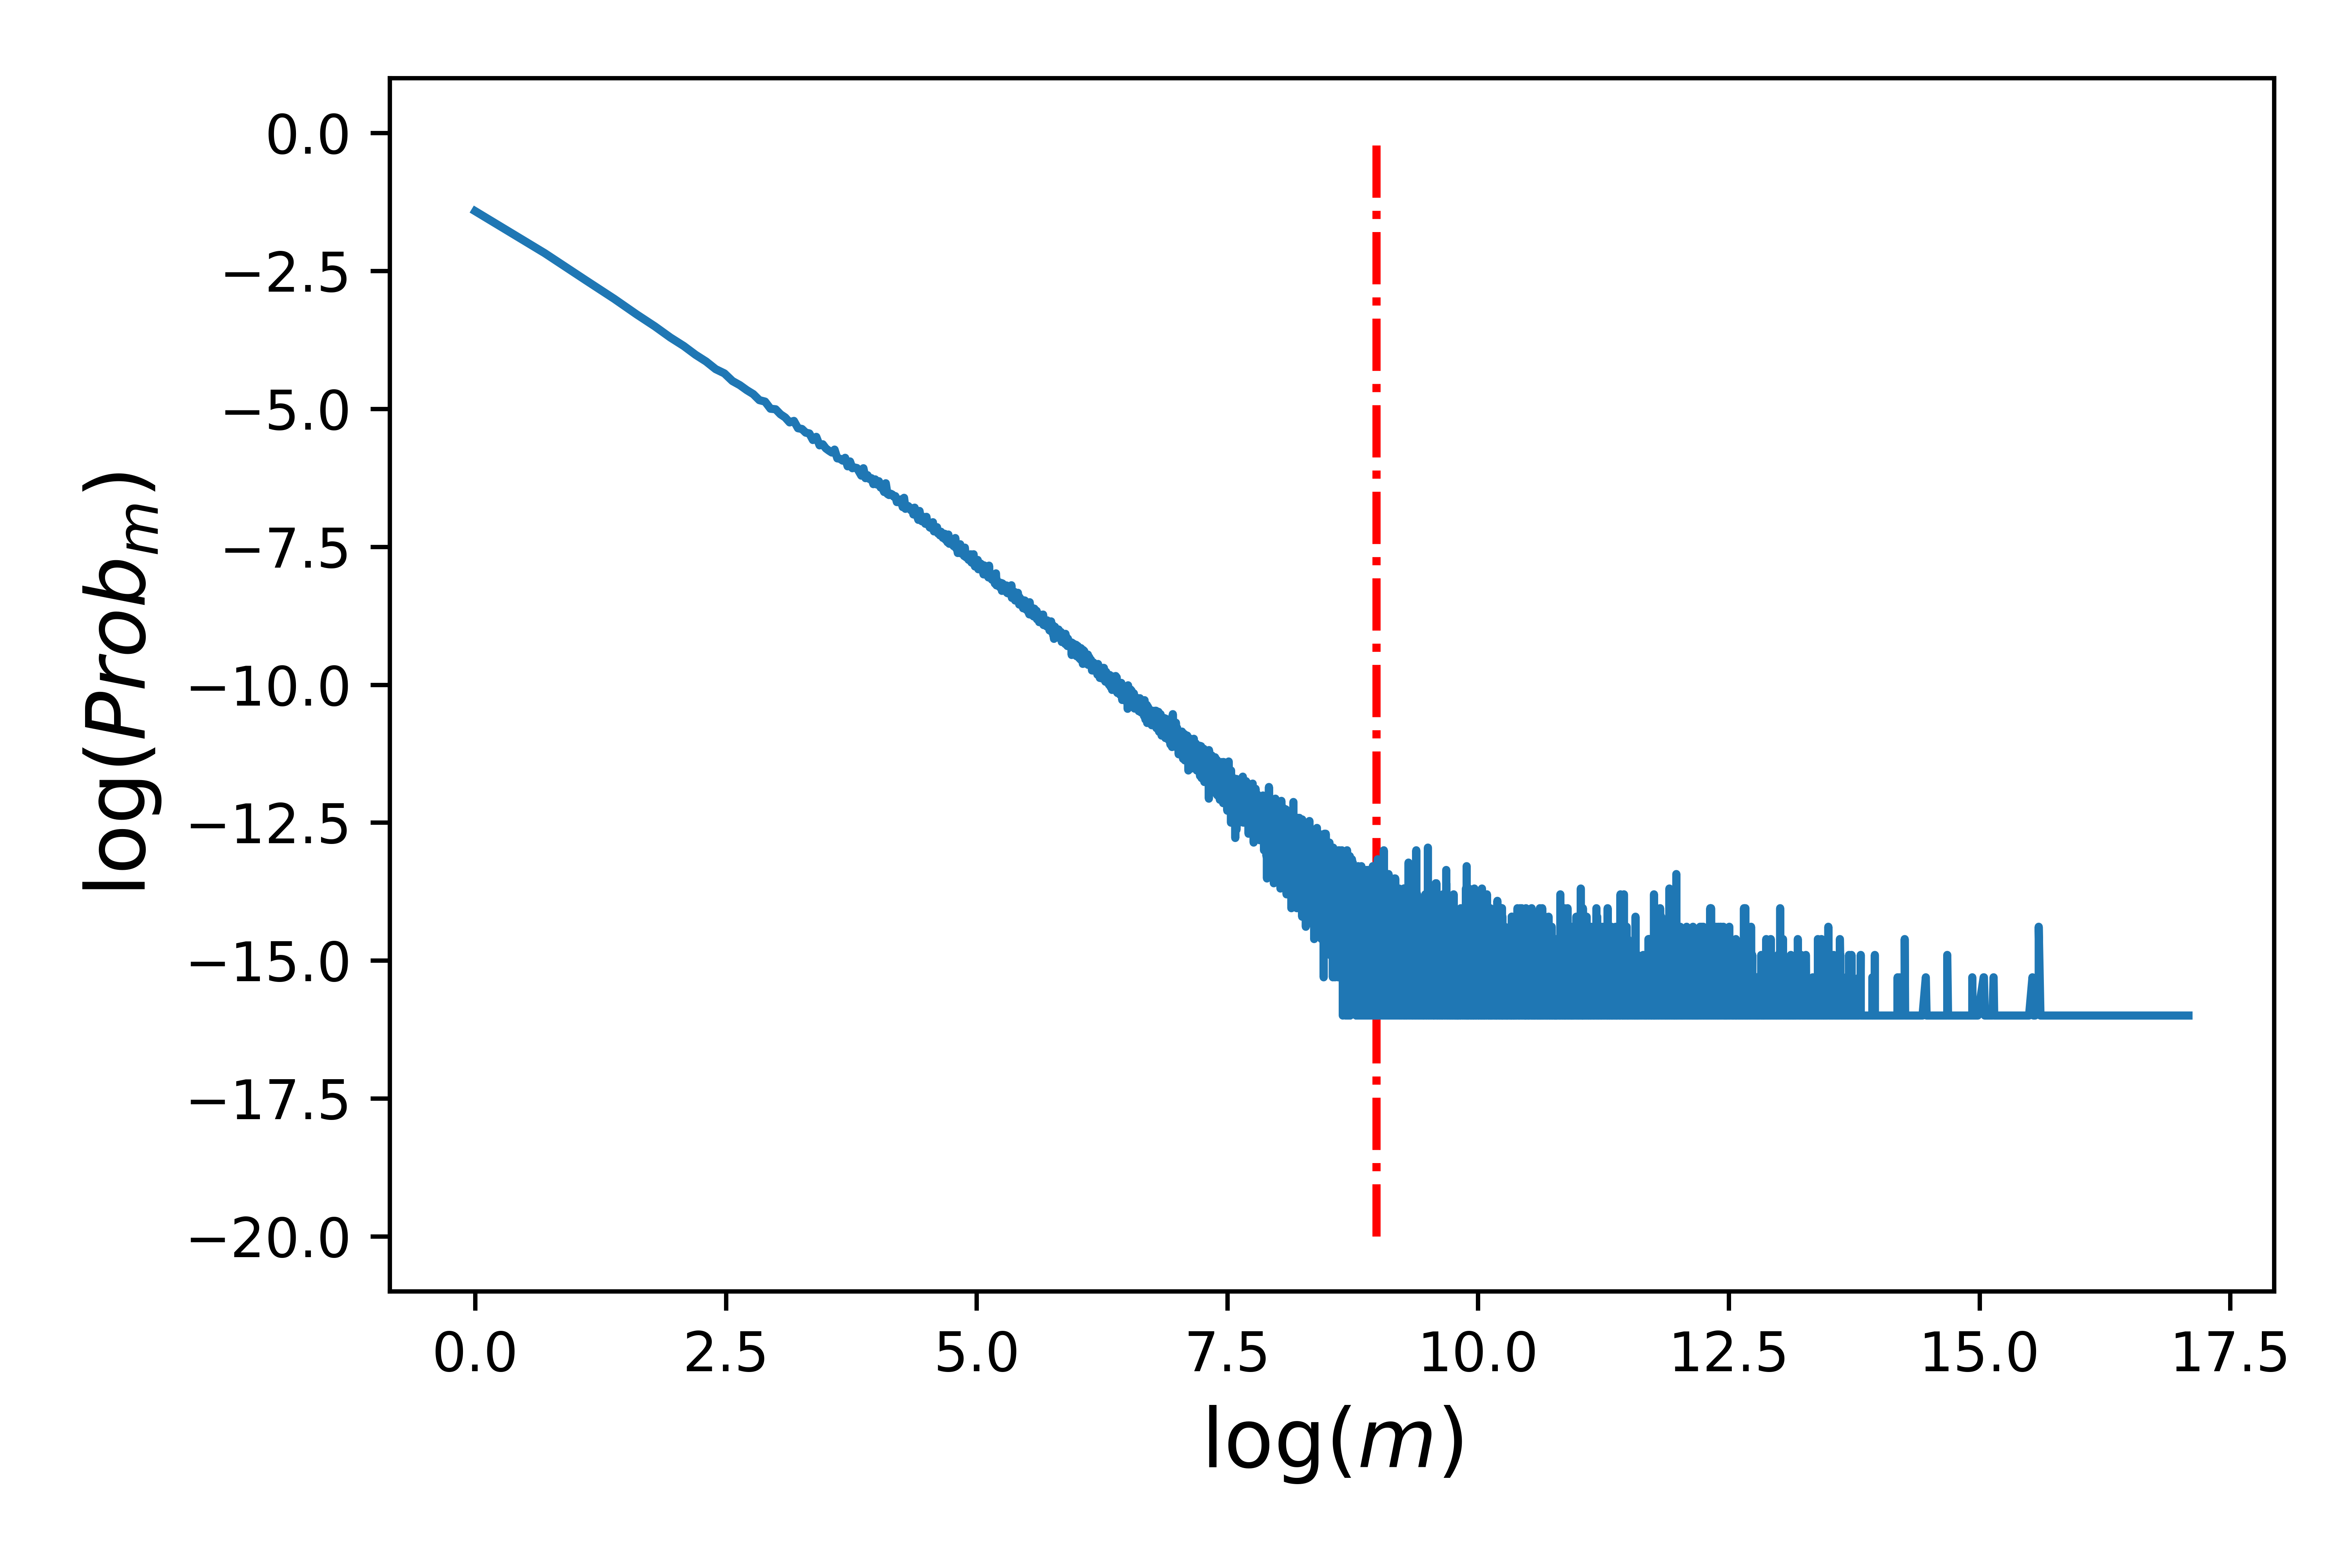
\includegraphics[width=1\textwidth]{avazu-thresh.png}
		\end{minipage}
	}
	\subfigure[Company set]{
	\begin{minipage}[b]{0.5\textwidth}
		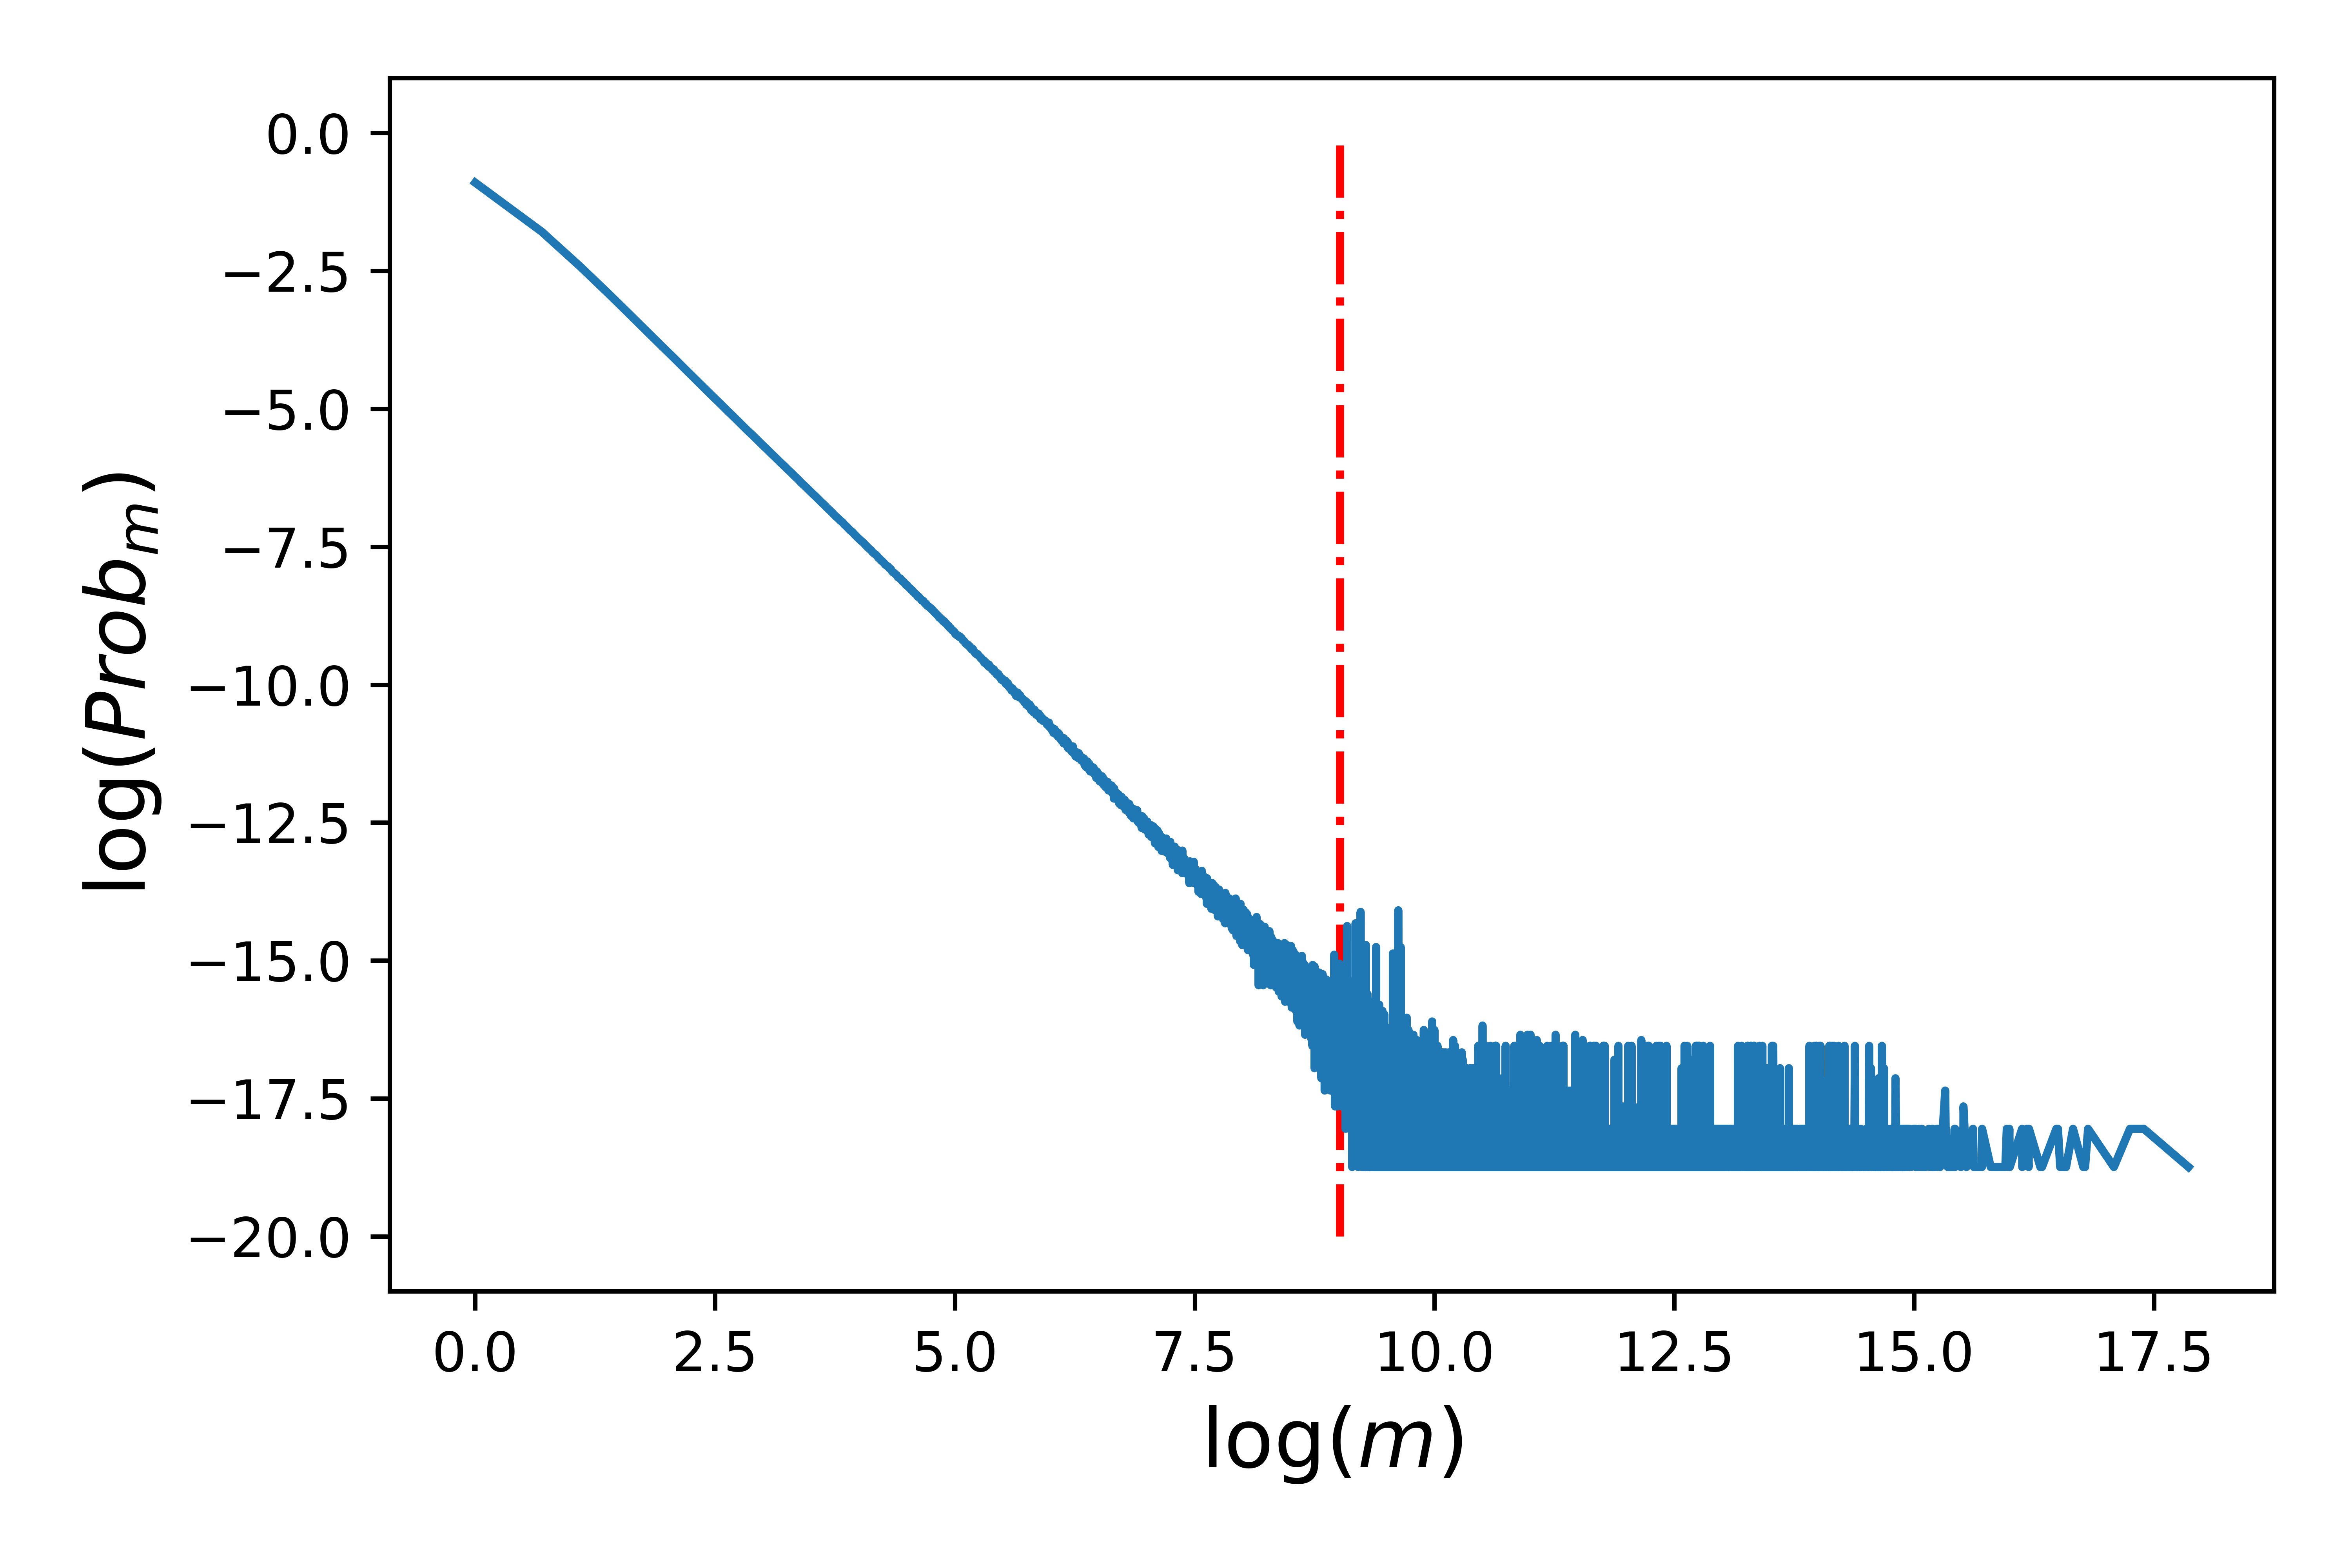
\includegraphics[width=1\textwidth]{hw-thresh.png}
	\end{minipage}}
	\caption{Distribution of feature-pair frequency of Avazu and Company sets. Both axes are log-scaled. Vertical lines correspond to the optimal $val_{\text{thresh}}$ values used in Table \ref{tab2}.}
	\label{fig.2}
\end{figure}

\section{Experiments on General Classification Data}
While our motivation in developing the adaptive model is for CTR prediction, the same idea may be useful for general classification problems. While in Figures \ref{fig.1}-\ref{fig.2} dense and sparse feature pairs are well separated, it is important to check if the same situation occur for other data sets. Therefore, in this section we collect and evaluate the following three types of data.
\begin{itemize}
\item Fully dense: for every feature, values in all (or almost all) instances are non-zero.
\item Highly sparse: for every feature, the number of non-zero values is very small.
\item Both: some features in the set are very dense, while others are highly sparse.
\end{itemize}
{\bf Describe our selected data sets,}
{\bf describe training, validation and test sets preparation,}
{\bf maybe we run Poly2 and FM rather than FFM because we may not have field information.}

Data statistics are in Table\ref{Table3}.
{\bf Table\ref{Table3} can present Data set Num:... Num:... Num:dense features Num:sparse features.}
{\bf issue: should we use logloss or accuracy?}

The parameter selection procedure is the same as that in Section \ref{sec:comparition}.{\bf Parameter ranges may need to by different?}

\section{Related work}
Our research provides a novel perspective of feature interaction and improves the CTR prediction. The most related domains are focused learning and feature interaction related models for CTR prediction. We will review studies of these two domains.

One closely related domain is a novel learning regime, named focused learning \cite{Beutel:2017:BGO:3038912.3052713} proposed by Google. To solve the ill-served items in recommendation, they divide the set of items into different subsets according to different objectives. They further conduct many experiments to demonstrate the effectiveness. Other related works include that some learn local models \cite{Christakopoulou:2016:LIM:2959100.2959185}, and some ensemble local learners \cite{Beutel:2015:AAC:2736277.2741091}. Our study is inspired by focused learning, but we focus on different ways for adaptively modeling feature conjunction.

CTR prediction plays an important role in recommendation. Many machine learning models have been proposed for this task. Google \cite{McMahan:2013:ACP:2487575.2488200} reported that their CTR prediction system is based on an online learning algorithm to learn a linear model. Their algorithm follows from the method follow-the-regularized-leader (\text{FTRL}) \cite{pmlr-v15-mcmahan11b}. Unlike a linear model, Facebook \cite{He:2014:PLP:2648584.2648589} provides a tree-based model for their CTR prediction system, in which the tree model is served as a way for feature engineering. Many CTR prediction models are proposed based on FM \cite{5694074}. We briefly discuss some of them. A tensor based model \cite{Rendle:2010:PIT:1718487.1718498} is used in personalized tag recommendation. FFM \cite{Juan:2016:FFM:2959100.2959134} has been proven to be an effective model in real CTR advertising system \cite{Juan:2017:FFM:3041021.3054185}. Difacto \cite{Li:2016:DDF:2835776.2835781} is the first one that expands FM to large-scale machine learning systems. Instead of using a fixed $k$ as the length of the latent vector, Difacto introduces the memory adaptive constraint, making the value $k$ depend on a single feature frequency. In terms of feature-pair interactions, AFM \cite{ijcai2017-435} is proposed to solve the weights of feature interactions via attentional networks. Starting from a bad case in FM, \cite{Prillo:2017:EVF:3109859.3109892} provides an elementary view on FM and also discusses issues of feature conjunction in FM. With the deep learning method, DeepFM \cite{Guo:2017:DFB:3172077.3172127} learns more sophisticated feature interactions. Different from these studies, our data adaptive model provides a novel insight on feature conjunction. The proposed model shows an improved CTR prediction on different real data sets.

\section{Conclusion}
In this paper, we proposed a model-based feature conjunction framework. Under this general framework, an adaptive model based on feature-pair frequency is used to improve the CTR prediction in recommender systems. The main idea is to apply the most suitable model for each pair of feature conjunction. While the concept is extremely simple, the selection of models depends on some hyperparameters. We demonstrate that with a proper design of the parameter-selection procedure, a right selection or combination of models can be achieved for CTR prediction problems. We conducted extensive experiments on two sets from Kaggle competitions and a Company data set from our production system to compare our model and the state-of-the-art models. The experimental results suggest our model is effective in predicting CTR.

Although the proposed method proves the success of model-based feature conjunction, there are still some interesting works for further studies. As to the framework, one future direction is to explore the combination of more models for CTR prediction. Another direction is to check different ways of feature conjunction. Besides, we will conduct further online experiments to evaluate effectiveness of our model.
\bibliographystyle{ACM-Reference-Format}
\bibliography{ffmpoly2-ref}
\end{document}


